\documentclass{ximera}

\title{Points of Interest on Graphs - Discontinuities}
\begin{document}
\begin{abstract}
    This section describes discontinuities of a function as points of interest (PoI) on a graph.
\end{abstract}
\maketitle


\subsection*{Discontinuities of a function}
    
    Here is a video!
    
    \youtube{Eko1Cgp-ECQ}
    
    Discontinuities originate in a variety of ways and are a topic of extensive study at several levels of mathematics. The nature of a given discontinuity can be informative about what is happening either within the model (eg the model is failing to properly represent reality at a specific point), or within the context of the model (some naturally occurring phenomena that the model is somehow 'capturing' and representing as a discontinuity). 
    
    For example; discontinuities occur in models of the formation of black holes where the singularity is formed because the density of matter at the singularity is going to infinity. Discontinuities also appear in the basics of quantum mechanics because of how the collapse of probability fields work at a quantum level, and even (simplified) models of objects traveling through the air and colliding with surfaces have discontinuities!
    
    There are three types of discontinuities:
    \begin{description}
        \item[\textbf{Holes:}] Holes are when a function seems to be nice and continuous, but is lacking a single point somewhere in the domain causing a small ``hole'' in the graph. This is typically represented by an unfilled circle around the missing point. Below is an example of a hole discontinuity at $(4,2)$:
        \begin{center}
            \begin{tikzpicture}
                \begin{axis}[axis x line=middle, 
                        axis y line=middle, 
                        xlabel={$x$}, 
                        ylabel={$y$}, 
                        axis equal, 
                        xtick={-1,0,...,8,9}, 
                        ytick={-2,-1,...,4},
                        xmin=-1, xmax=9.5, 
                        ymin=-3, ymax=3.5]
                    \addplot[-,domain=0:4, samples=300]{x^(1/2)};
                    \addplot[->,domain=4:9, samples=300]{x^(1/2)};
                    \addplot[mark=*,white] coordinates{( 4,2)};% Used 1.386294 instead of ln(4) because pgfplots is bitchy.
                    \addplot[mark=o] coordinates{( 4,2)};% Used 1.386294 instead of ln(4) because pgfplots is bitchy.
                \end{axis}
            \end{tikzpicture}
        \end{center}
        \item[\textbf{Asymptotic (Infinite):}] Asymptotic (sometimes called `infinite') discontinuities are when the function bends up or down and approaches a vertical asymptote as it gets close to the point of discontinuity. This typically demonstrates that something very strange is happening, since reality rarely tries to push something to `infinity'; so typically an infinite discontinuity is a sign that your model is either capturing a truly spectacular moment (like the formation of a singularity in a black hole), or you are trying to do something you \textit{really} shouldn't be trying to do with that model, like when stock market algorithms cause chaotic feedback and create unstable markets.%
            \footnote{%
                This is one of the reasons some experts think that the so-called `flash-crash of May 6th' occurred, in which the stock market dropped over 9\% (about 1 \textit{trillion} dollars in value), only to spontaneously pop back up 36 minutes later.%
                }
        Below is an example of a asymptotic (aka infinite) discontinuity:
        \begin{center}
                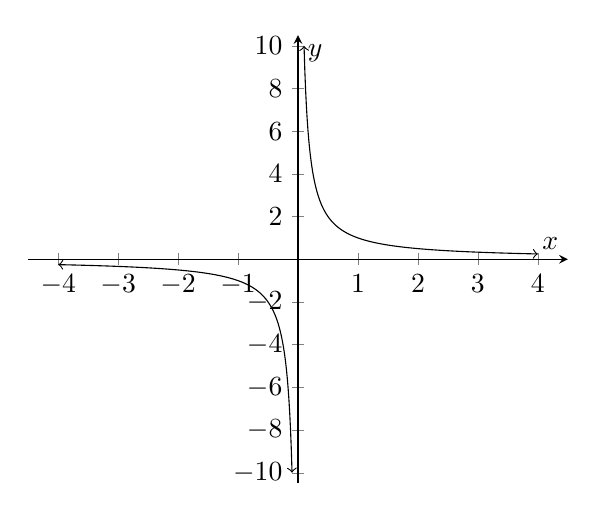
\begin{tikzpicture}
                    \begin{axis}[axis x line=middle, 
                            axis y line=middle, 
                            xlabel={$x$}, 
                            ylabel={$y$},
                            xtick={-4,-3,...,3,4}, 
                            ytick={-10,-8,...,10},
                            xmin=-4.5, xmax=4.5, 
                            ymin=-10.5, ymax=10.5]
                        \addplot[<->,domain=-4:-0.1, samples=300]{1/x};
                        \addplot[<->,domain=0.1:4, samples=300]{1/x};
                    \end{axis}
                \end{tikzpicture}
            \end{center}
                    
        \item[\textbf{Jump:}] Jump discontinuities occur when the function suddenly `jumps' from one value to another without covering the space between. This typically happens because the model is either not inherently continuous (eg the model is rounding to the nearest whole number, so it will skip from one whole number to the next without hitting any numbers between), or some sort of important threshold in the model's context is being hit, such as entering a new tax bracket when calculating taxes. Below is an example of a jump discontinuity:
        \begin{center}
                \begin{tikzpicture}
                    \begin{axis}[axis x line=middle, 
                            axis y line=middle, 
                            xlabel={$x$}, 
                            ylabel={$y$}, 
                            axis equal, 
                            xtick={-1,0,...,8,9}, 
                            ytick={-2,-1,...,4},
                            xmin=-1, xmax=9.5, 
                            ymin=-3, ymax=3.5]
                        \addplot[-,domain=0:4, samples=300]{x^(1/2)};
                        \addplot[->,domain=4:9, samples=300]{ln(x)};
                        \addplot[mark=*] coordinates{(4,2)};
                        \addplot[mark=*,white] coordinates{( 4,1.386294)};% Used 1.386294 instead of ln(4) because pgfplots is bitchy.
                        \addplot[mark=o] coordinates{( 4,1.386294)};% Used 1.386294 instead of ln(4) because pgfplots is bitchy.
                    \end{axis}
                \end{tikzpicture}
            \end{center}
    \end{description}

    \begin{problem}
        What is the importance of discontinuities?
        \begin{multipleChoice}
            \choice[correct]{Discontinuities represent the places where your function (and thus your model) is behaving in a weird way; which suggests further study may be worthwhile.}
            \choice{Discontinuities represent where your model is broken, and thus you should create a new/improved model to remove them.}
            \choice{Discontinuities are important in other areas of math, so we should learn them now.}
            \choice{Discontinuities aren't ever useful in the real world, so they don't have importance outside of the classroom.}
        \end{multipleChoice}
    \end{problem}

\end{document}